\documentclass[8pt]{beamer}
\usepackage[utf8]{inputenc}

\usepackage{blindtext}
\usepackage{lipsum}
\usepackage{multirow}
\usepackage{amsmath}
\usepackage{url}
\usepackage[russian]{babel}
\usepackage{listings}
\usepackage{hyperref}
\usepackage{bbm}
\graphicspath{{images/}}


\title[Разработка технологии ДНК-идентификации]{Разработка технологии ДНК-идентификации и определения этногеографической принадлежности неизвестного индивида}
\author[Демидко Д. А.]{Демидко Дмитрий Андреевич}
\institute[]{{\footnotesize\bfseries БЕЛОРУССКИЙ ГОСУДАРСТВЕННЫЙ УНИВЕРСИТЕТ\\ \vspace{.5em} Кафедра дискретной математики и алгоритмики}}
\date{}
\centering
\begin{document}

\begin{frame}
\vfill
\centering

\begin{beamercolorbox}[sep=8pt,center,colsep=-4bp,rounded=true,shadow=true]{institute}
\usebeamerfont{institute}\insertinstitute
\end{beamercolorbox}

\vspace{0.5em}\par

{\usebeamercolor[fg]{titlegraphic}\inserttitlegraphic\par}

\begin{beamercolorbox}[sep=8pt,center,colsep=-4bp,rounded=true,shadow=true]{author}
\usebeamerfont{author}\insertauthor
\end{beamercolorbox}

\vspace{0.5em}\par

\begin{beamercolorbox}[sep=8pt,center,colsep=-4bp,rounded=true,shadow=true]{title}
\usebeamerfont{title}\inserttitle\par%
\ifx\insertsubtitle\@empty%
\else%
\vspace{0.25em}%
{\usebeamerfont{subtitle}\usebeamercolor[fg]{subtitle}\insertsubtitle\par}%
\fi%
\end{beamercolorbox}%

\vspace{1.5em}\par

{\centering\bfseries\small Научный руководитель\\\vspace{0.5em}}
{\centering\small Андрианов Александр Михайлович\\ \vspace{0.3em}}
{\centering\itshape\small доктор химических наук, профессор кафедры БМИ ФПМИ\\}

\vspace{1em}\par

\begin{beamercolorbox}[sep=8pt,center,colsep=-4bp,rounded=true,shadow=true]{date}
\usebeamerfont{date}\insertdate
\end{beamercolorbox}\vspace{0.5em}

\end{frame}

\begin{frame}{Введение}
    \begin{block}{Представленная магистерская диссертация посвящена разработке технологии ДНК-идентификации.}
    \end{block}

    \begin{block}{}
        Основная часть представленной магистерской диссертации включает в себя 4 главы.
        В первой главе работы приводятся некоторые понятия связанные с геномикой,
        а также общая схема схема ДНК-идентификации.
        Вторая глава работы посвящена обработке последовательностей нуклеотидов полученных в результате
        сенирование геномов, нахождению STR-маркеров, поиску возможных шаблонов STR-маркеров,
        а также аннотации STR-маркеров.
        Третья глава посвящена определению этногеографической принадлежности индивидов на основе ДНК-маркеров на территории Республии Беларусь.
        Четвертая глава содержит описание разработанных методов по определению географической принадлежности индивидов на основе ДНК-маркеров на территории Республии Беларусь.
    \end{block}
\end{frame}

\begin{frame}{Глава 1, Раздел 2}
    \begin{block}{Общая схема ДНК-идентификации}
        \begin{itemize}
            \item Получение, хранение биоматериалов
            \item Секвенирование генома, отдельных хромосом, специальных участков
            \item \textbf{Аннотация секвенированных последовательностей на основе референсной информации}
            \item \textbf{Анализ полученных генотипов}
        \end{itemize}
    \end{block}
\end{frame}

\begin{frame}{Глава 2, Раздел 1}
    \begin{block}{Подготовка файлов}
        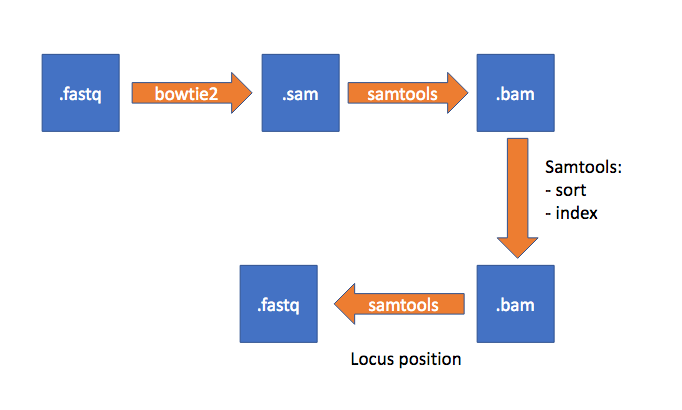
\includegraphics[height=6.8cm]{images/locus_r.png}
        \centering
    \end{block}
\end{frame}

\begin{frame}{Глава 2, Раздел 2}
    \begin{block}{Поиск STR-маркеров в прочтениях}
        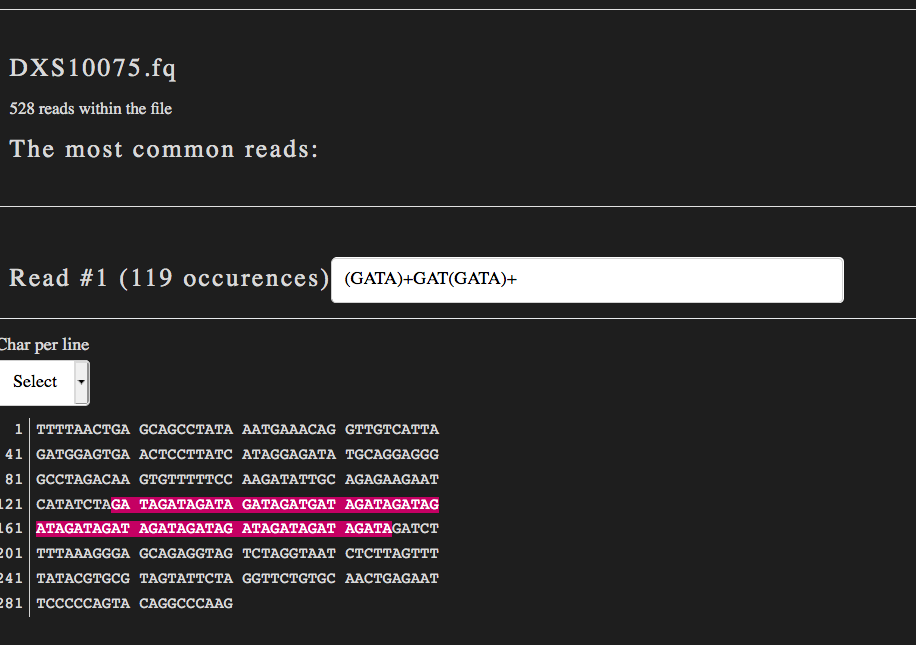
\includegraphics[height=6.8cm]{images/str_search.png}
        \centering
    \end{block}
\end{frame}

\begin{frame}{Глава 2, Раздел 3}
    \begin{block}{Поиск шаблонов STR-маркеров}
        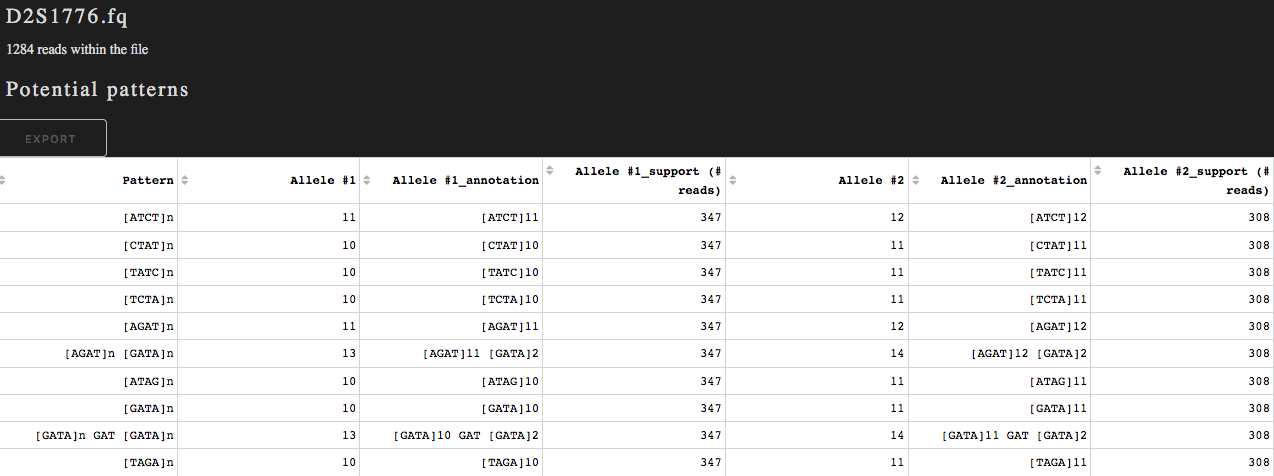
\includegraphics[height=6.8cm]{images/str_pat_search.png}
        \centering
    \end{block}
\end{frame}

\begin{frame}{Глава 2, Раздел 4}
    \begin{block}{Аннотация STR-маркеров}
        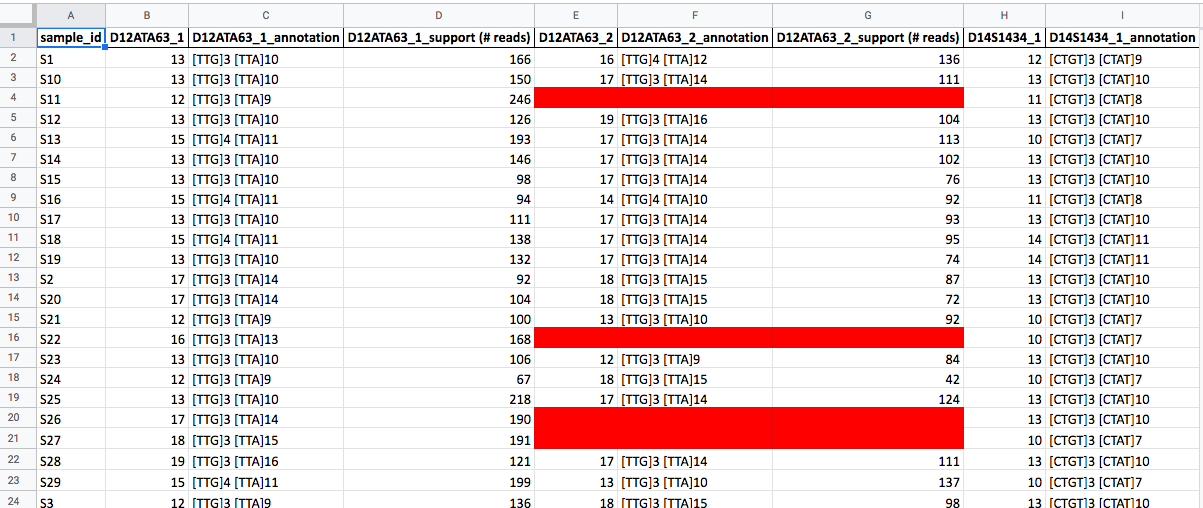
\includegraphics[height=6.8cm]{images/ann.png}
        \centering
    \end{block}
\end{frame}

\begin{frame}{Глава 2, Раздел 4}
    \begin{block}{Аннотация STR-маркеров}
        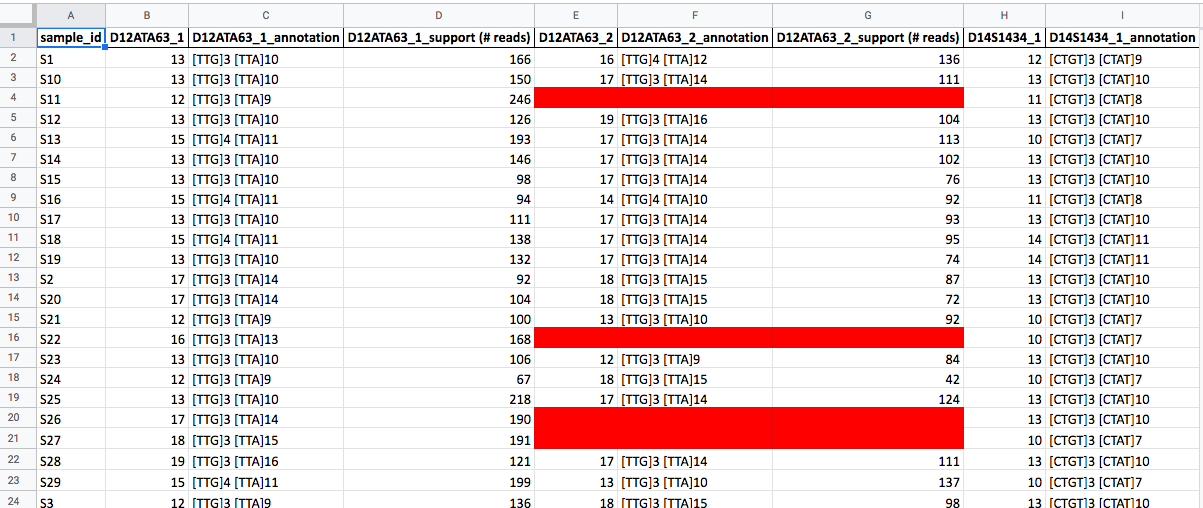
\includegraphics[height=6.8cm]{images/ann.png}
        \centering
    \end{block}
\end{frame}

\begin{frame}{Глава 3, Раздел 1}
    \begin{block}{Исправление ошибок в размеченных данных}
        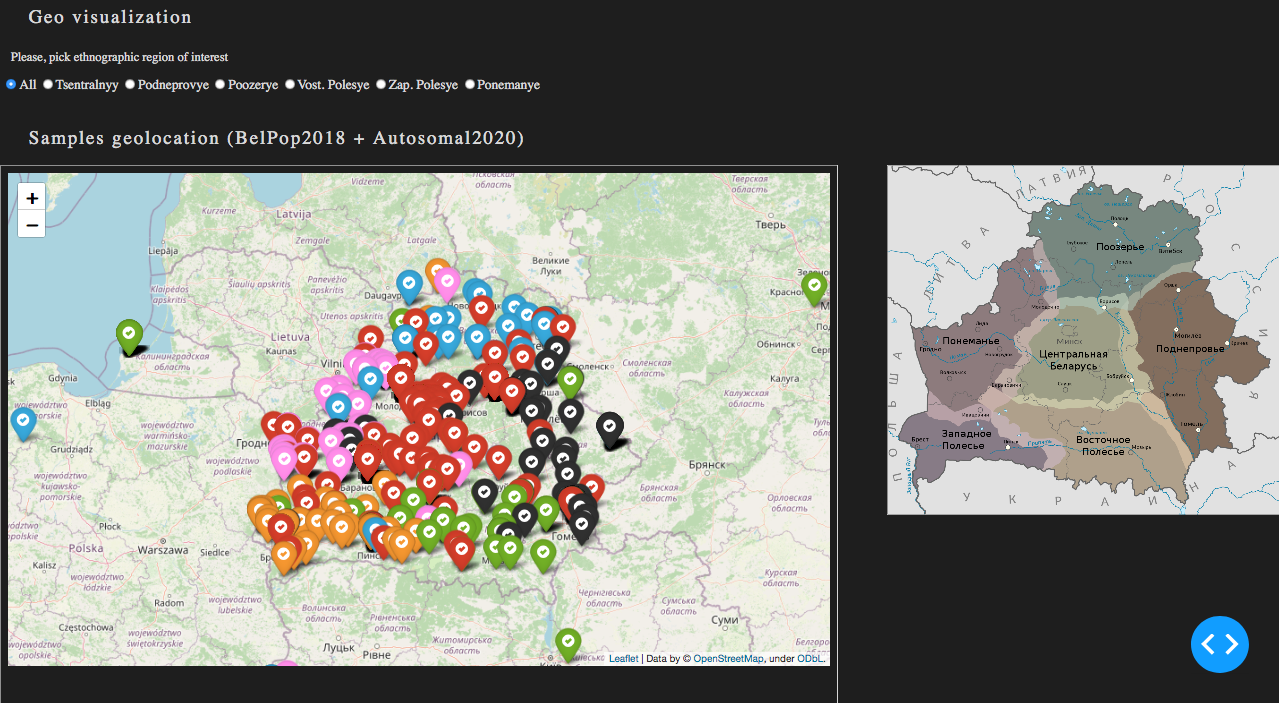
\includegraphics[height=3.8cm]{images/geomap_v1.png}
        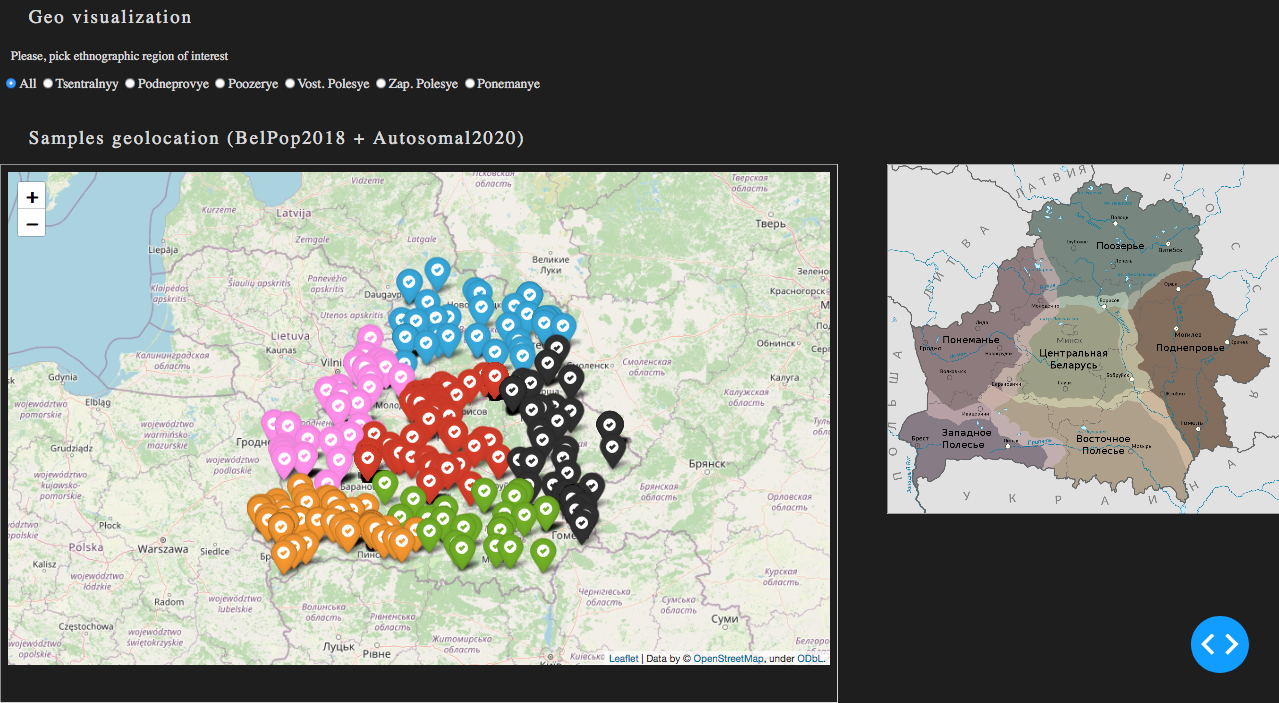
\includegraphics[height=3.8cm]{images/geomap_v2.png}
        \centering
    \end{block}
\end{frame}

\begin{frame}{Глава 3, Раздел 2}
    \begin{block}{Использованная методология обучения моделей}
        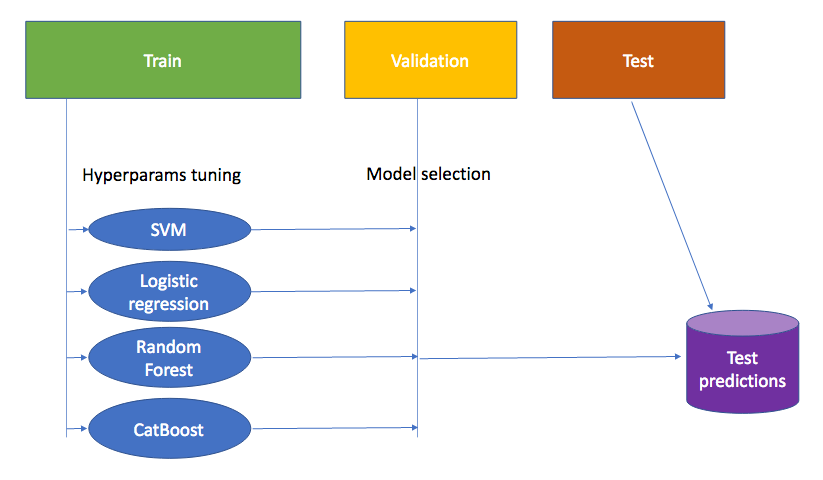
\includegraphics[height=6.8cm]{images/ml_info.png}
        \centering
    \end{block}
\end{frame}

\begin{frame}{Глава 3, Раздел 2}
    \begin{block}{Качество классификации генотипов для этногеографической принадлежности}
        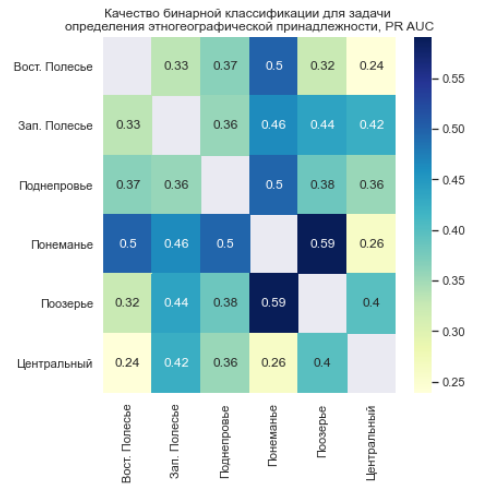
\includegraphics[height=6.8cm]{images/bel_reg_pr_auc.png}
        \centering
    \end{block}
\end{frame}

\begin{frame}{Глава 3, Раздел 2}
    \begin{block}{Качество классификации генотипов на уровне рас}
        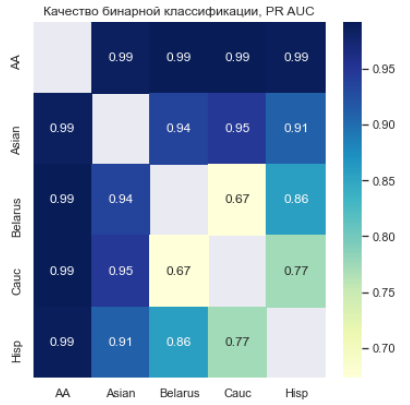
\includegraphics[height=6.8cm]{images/bel_us_pr.png}
        \centering
    \end{block}
\end{frame}

\begin{frame}{Положения, выносимые на защиту}
    \begin{itemize}
        \item Метод генерации шаблонов для STR-маркеров
        \item Метод аннотации для STR-маркеров
        \item Модели машинного обучения для определения этногеографической принадлежности по генотипу
    \end{itemize}
\end{frame}


\begin{frame}
\huge{\centerline{Спасибо за внимание!}}
\end{frame}

\end{document}
